\documentclass[a4paper,11pt,oneside]{book}

% PACCHETTI
\usepackage{hyperref}           % hyperlinks
\usepackage{tabto}              % strumento per inserire tab nel testo
\usepackage[                    % geometria della pagina
    a4paper,
    inner=2cm,
    outer=3cm,
    top=3cm,
    bottom=3cm,
    bindingoffset=1.2cm,
    headheight=14pt
]{geometry}
\usepackage[utf8]{inputenc}     % 3 pacchetti per l'italiano
\usepackage[italian]{babel}
\usepackage[T1]{fontenc}
\usepackage{titlesec}           % custom chapter titles

\usepackage{fancyhdr}
\usepackage{multicol}
\usepackage[arrowdel]{physics} 
\usepackage{amsmath}
\usepackage{tikz}

\usepackage{graphicx}           % IMMAGINI
\graphicspath{ {./images/} }
\usepackage{wrapfig}

\usepackage{csquotes}
\usepackage{caption}

\usepackage{listings}
%\usepackage{minted}

% INFORMAZIONI SUL DOCUMENTO
\title{\Large{\textbf{Programmazione 1}}}
\author{Enrico Bragastini}
\titleformat{\chapter}[display]{\normalfont\bfseries}{}{0pt}{\LARGE}


% CONTENUTO
\begin{document}
\pagestyle{fancy}
\fancyhf{}
\rhead{}
\lhead{\nouppercase\leftmark}
\cfoot{\thepage}
\frontmatter

% Prima pagina - Titolo
\maketitle
\tableofcontents

\mainmatter
\chapter{Stringhe}
Una stringa è un \emph{array di caratteri} terminato dal carattere '\textbackslash0'.
Quindi dichiarando una stringa lunga 20 caratteri, saranno 19+1 dove l'ultimo è il carattere di terminazione.

\section{Dichiarazione di una stringa}
Dichiarazione di una stringa come array di lunghezza 20 caratteri:
\begin{lstlisting}[language=C]
    char stringa[20]; 
\end{lstlisting}

~\newline
Dichiarazione di una stringa e inizializzazione del suo contenuto:
\begin{lstlisting}[language=C]
    char stringa[20] = "ciao, tutto bene?"; # 17+1 caratteri
\end{lstlisting}
in questo caso viene allocato uno spazio sufficiente per 20 caratteri, ma ne vengono utilizzati solamente 18.

\section{Lettura di una stringa}
Con lo \textbf{scanf} si può leggere un array di caratteri senza avere bisogno di un ciclo. Viene inserito automaticamente 
un '\textbackslash0' alla fine della stringa. Leggerà fino a trovare uno spazio oppure un andata a capo.

\begin{lstlisting}[language=C]
    scanf("%s", stringa);
\end{lstlisting}
Per leggere stringhe anche con spazi o con andate a capo si può utilizzare gets. Gets è pericoloso perché può leggere anche stringhe più lunghe dello spazio allocato.
\begin{lstlisting}[language=C]
    gets(stringa);
\end{lstlisting}
Il modo corretto è leggere stringhe con spazi è mediante un ciclo:
\begin{lstlisting}[language=C]
    int i;
    i = 0;
    do{
        scanf("%c", &stringa[i]);
        i++;
    } while(stringa[i-1] != '\n');
    stringa[i-1] = '\0'
\end{lstlisting}

\section{Libreria string.h}
Alcune funzioni dalla libreria \emph{string.h} utili per eseguire operazioni con le stringhe:
\begin{itemize}
    \item STRLEN: restituisce la \textbf{lunghezza} di una stringa senza il '\textbackslash0'
    \item STRCMP: \textbf{compara} due stringhe, restituendo un intero che vale $0$ se le stringhe sono uguali, $-1$ se $S1<S2$ e 1 se $S1>S2$.
    \item STRCPY: \textbf{copia} il contenuto di $S2$ in $S1$
    \item STRCAT: restituisce la \textbf{concatenazione} di $S2$ a $S1$
\end{itemize}

\chapter{Struct}
Le \emph{Struct} sono delle variabili strutturate, ovvero degli aggregati di campi, utilizzate per 
memorizzare informazioni non omogenee di tipo. Hanno la seguente forma:
\begin{lstlisting}[language=C]
    struct{
        # campi
    } <nome>;
\end{lstlisting}

\section{Esempio e dimensione di una Struct}
Esempio di Struct per memorizzare delle informazioni di uno studente:
\begin{lstlisting}[language=C]
    struct{
        char matricola[6];
        char nome[20+1];
        char cognome[20+1];
        float media;
    } studente;
\end{lstlisting}
La dimensione di questa variabile equivale quindi a
\begin{equation*}
    6 \times 8 \;\text{bit} +
    21 \times 8 \;\text{bit} +
    21 \times 8 \;\text{bit} +
    1 \times 32 \;\text{bit} = 416 \; \text{bit}
\end{equation*}

\section{Usare le struct}
Per accedere alle variabili interne di una Struct si usa la seguente sintassi:
\begin{lstlisting}[language=C]
    struct.variabile
\end{lstlisting}

~\newline
Esempio di lettura e scrittura:
\begin{lstlisting}[language=C]
    printf("Inserire il voto medio");
    scanf("%f", &studente.media);
    printf("Voto medio: ", studente.media);

    int i;
    for(i=0; i<6; i++){
        scanf("%c", &studente.matricola[i]);
    }
\end{lstlisting}

~\newline
È possibile dichiarare più struct in un colpo solo:
\begin{lstlisting}[language=C]
    struct{
        # campi
    } <nome1>, <nome2>;
\end{lstlisting}
ed è possibile copiare una struct con un'altra come si farebbe per una normale variabile:
\begin{lstlisting}[language=C]
    struct1 = struct2;
\end{lstlisting}
questo copierà rispettivamente tutti i campi di \emph{struct2} dentro a \emph{struct1}

\section{Struct per creare nuovi tipi di variabili}
Dichiarando una struct come segue:
\begin{lstlisting}[language=C]
    struct info{
        int min;
        int max
    };
\end{lstlisting}
verrà creato un nuovo tipo di variabile. Sarà quindi possibile dichiarare variabili di tipo \textbf{info}.
Per essere utilizzato il tipo \textbf{info}, è necessaria anche la keyword \textbf{struct}. Quindi per 
dichiarare due variabili \emph{a} e \emph{b} di tipo \emph{info}, bisognerà scrivere
\begin{lstlisting}[language=C]
    struct info a, b;
\end{lstlisting}

\subsection{Typedef}
Esiste in C un'istruzione che permette di creare dei nuovi tipi di variabili, l'istruzione \textbf{tupedef}.
\begin{lstlisting}[language=C]
    typedef int mio_int; 
\end{lstlisting}
Scrivendo un'istruzione del genere, creiamo un nuovo tipo, chiamato \emph{mio\_int}, che è un \emph{alias} del tipo \emph{int}.

Questa istruzione risulta particolarmente utile per creare delle nuove tipologie di variabili, in combinata con le \emph{struct}.
Vediamo un esempio:
\begin{lstlisting}[language=C]
    typedef struct{
        int min;
        int max;
    } t_info; 
\end{lstlisting}
Così facendo avremo creato una variabile \textbf{user-defined} di tipo \emph{t\_info}.
Potremo quindi scrivere
\begin{lstlisting}[language=C]
    t_info a, b;
\end{lstlisting}
per dichiarare due variabili di tipo \emph{t\_info}

\chapter{Puntatori}
Un puntatore è una \emph{variabile} che contiene l'\textbf{indirizzo} di un'altra variabile.

\section{Dichiarazione di un puntatore}
Un puntatore si dichiara specificando il tipo della variabile a cui si sta puntando e il nome del puntatore stesso:
\begin{lstlisting}[language=C]
    int *p;
\end{lstlisting}

Supponiamo quindi di avere una variabile intera \textbf{a} e il puntatore \textbf{p}. Vogliamo che il puntatore contenga l'indirizzo della 
variabile a:
\begin{lstlisting}[language=C]
    int main(){
        int a;
        int *p;
        a = 5;
        p = &a;     // assegnazione di p
        return 0;
    } 
\end{lstlisting}
È possibile ora andare a modificare il valore della variabile \textbf{a} accedendovi sia tramite la stessa variabile \textbf{a}, che tramite il puntatore \textbf{p}:
\begin{lstlisting}[language=C]
    a++;
    (*p)++;
\end{lstlisting}

\section{Operatori}
Per lavorare con i puntatori si utilizzano due operatori:
\begin{itemize}
    \item \textbf{*}: L'\emph{asterisco} è detto operatore di \emph{deferenziazione}. Permette di lavorare con la variabile puntata dal puntatore.
    \item \textbf{\&}: Il simbolo \emph{E-commerciale} permette di riferirsi all'indirizzo di una variabile.
\end{itemize}

~\newline
Esempio:
\begin{lstlisting}[language=C]
    int main(){
        int i = 5, j = 9;
        int *p;
        p = &j;     // p punta alla variabile j
        *p = i;     // viene modificato il valore di j
    }
\end{lstlisting}

\section{Puntatore a puntatore}
È possibile anche creare dei puntatori a dei puntatori.

~\newline Esempio:
\begin{lstlisting}[language=C]
    int main(){
        int c, d;
        int *p1;
        int *p2;
        int **p3;
        int **p4;
        ...
    }
\end{lstlisting}
Le variabili create sono:
\begin{itemize}
    \item \textbf{c} e \textbf{d}: variabili intere 
    \item \textbf{p1} e \textbf{p2}: puntatori a variabili intere 
    \item \textbf{p3} e \textbf{p4}: puntatori a puntatori a variabili intere
\end{itemize}
Se si andasse ad aggiungere il seguente codice:
\begin{lstlisting}[language=C]
    c = 54;
    d = 10;
    p1 = &c;
    p2 = p1;
    printf("%d %d %d %d",c,d,*p1,*p2);
\end{lstlisting}
verrebbe stampata la stringa "54 10 54 54".
\begin{lstlisting}[language=C]
    p1 = &d;
    *p1 = *p1 + *p2:
    p3 = &p1;
    p4 = &p2;
    *p4 = *p3;
    printf("%d %d %d %d",c,d,*p1,*p2);
\end{lstlisting}
ora verrebbe stampata la stringa "54 64 64 64".

\section{Relazione tra array e indirizzi di memoria}
Vediamo alcune relazioni che ci sono tra gli array e gli indirizzi di memoria.
Sia dato un array n di 10 interi:
\begin{itemize}
    \item $n \; \equiv \; \&n[0]$
    \item $n+i \; \equiv \; \&n[i]$
    \item $*n \; \equiv \; *(\&n[0]) \; \equiv \; n[0]$
    \item $*(n+i) \; \equiv \; n[i]$
\end{itemize}

\chapter{File}
I file sono strutture di memoria permanenti. Vengono gestiti dal file system del Sistema Operativo. 
Il S.O. mette a disposizione dei processi la \textbf{tabella dei file aperti}, ovvero un \emph{array di strutture}.
Ogni cella di questo \emph{array} è di tipo \textbf{FILE} e contiene varie informazioni quali nome del file, modalità di accesso 
(lettura, scrittura, append...) puntatore alla posizione corrente indicatore di fine file\dots



\section{Sintassi}
Per lavorare con i file è necessario dichiarare un puntatore all'array FILE:
\begin{lstlisting}[language=C]
    FILE * fp;
\end{lstlisting}

~\newline
Per \textbf{aprire} un file si utilizza l'istruzione fopen:
\begin{lstlisting}[language=C]
    fp = fopen(nomefile, modalita);
\end{lstlisting}
dove la modalità può variare tra:
\begin{itemize}
    \item \textbf{r}: lettura
    \item \textbf{w}: scrittura
    \item \textbf{a}: append (scrittura dalla fine del file)
\end{itemize}

~\newline
È necessario assicurarsi che l'associazione del puntatore sia stata eseguita correttamente:
\begin{lstlisting}[language=C]
    if(fp){
        ...
    }
\end{lstlisting}

~\newline 
Per \textbf{scrivere} su file si usa la funzione \emph{fprintf}:
\begin{lstlisting}[language=C]
    fprintf(fp, "%d", num);
\end{lstlisting}

~\newline 
Per \textbf{leggere} da file si usa la funzione \emph{fscanf}:
\begin{lstlisting}[language=C]
    fscanf(fp, "%d", &num);
\end{lstlisting}

~\newline
Per \textbf{liberare} l'accesso al file è necessario usare la funzione \textbf{fclose}:
\begin{lstlisting}[language=C]
    fclose(fp);
\end{lstlisting}

\section{End of File}
La funzione \textbf{int feof(FILE * fp)} è una funzione molto utile per sapere se si è arrivati a leggere la fine del file.
La fine del file viene intercettata solamente dopo una lettura, quindi questa chiamata di funzione bisogna farla dopo aver letto almeno una volta dal file.
Questa funzione restituisce
\begin{itemize}
    \item Vero (1): è stata raggiunta la fine del file 
    \item Falso (0): non è stata raggiunta la fine del file
\end{itemize}

~\newline 
Esempio di lettura da file:
\begin{lstlisting}[language=C]
    int main(){
        int num;
        FILE * fp;
        if(fp){
            fscanf(fp, "%d", &num);
            while(!feof(fp)){
                printf("%d", num);
                fscanf(fp, "%d", &num);
            }
            fclose(fp);
        }
        else printf("Errore in lettura.");
    }
    
\end{lstlisting}

\chapter{Allocazione dinamica della memoria}
Fino ad ora abbiamo utilizzato una \emph{allocazione statica (automatica)} della memoria.
Con tale modalità le variabili vengono allocate automaticamente in memoria nello \textbf{stack} quando si entra in un blocco di codice (ad esempio una funzione)
e corrispondentemente vengono distrutte automaticamente quando si esce dal blocco stesso.

L'\textbf{allocazione dinamica} della memoria consente di determinare lo spazion necessario a certe variabili \textbf{durante l'esecuzione} del programma.
Una variabile viene allocata dinamicamente in memoria nello \textbf{heap} attraverso specifiche istruzioni, e rimane tale finché non viene \emph{esplicitamente} deallocata.

\section{Struttura della memoria}
La memorià è suddivisa nelle seguenti sezioni:
\begin{itemize}
    \item \textbf{Heap}: Zona separata che cresce nel verso opposto allo stack dove vengono allocati dinamicamente degli spazi di memoria di cui si conosce la dimensione
    solamente durante l'esecuzione del programma. È importante deallocare manualmente lo spazio precedentemente allocato.
    \item \textbf{Stack}: Sezione in cui vengono allocate le variabili locali automatiche. Per prime troviamo le variabili del \emph{main} e successivamente le variabili dei sottoprogrammi 
    chiamati. La dimensione dello stack dipende dal momento di esecuzione che si sta analizzando, questo perché alla fine di un sottoprogramma tutte le variabili non \emph{static} vengono deallocate automaticamente.
    \item \textbf{Global/Static variables}: Sezione in cui vengono caricate le variabili globali, visibili da tutte le funzioni e esterne al \emph{main}, e le variabili
     statiche (variabili locali di una funzione ma che mantengono il valore durante l'esecuzione)
    \item \textbf{Code}: Spazio di memoria in cui, nella fase di loading della catena di compilazoine del C, vengono caricate le istruzioni da eseguire.
\end{itemize}

\section{Funzioni calloc() e malloc()}
Le funzioni \textbf{calloc()} e \textbf{malloc()} della libreria standard \textbf{<stdlib.h>} consentono di allocare dinamicamente la memoria.

\subsection{calloc()}
La funzione calloc() richiede due argomenti che specificano: Il numero di elementi da riservare e la dimensione di ciascun elemento in byte.
Questa funzione restituisce poi un puntatore all'inizio dell'area di memoria allocata. Questo puntatore è di tipo \emph{void}, puntatore generico. Per essere
allocato alla variabile visogna eseguire un \emph{cast} di tipo.

L'area di memoria allocata viene automaticamente posta a 0.

\begin{lstlisting}[language=C]
    int *int_ptr;
    ... 
    int_ptr = (int *) calloc(1000, sizeof(int));
\end{lstlisting}


\subsection{malloc()}
La funzione malloc() richiede un solo argomento: il numero totale di byte da allocare in memoria. Restituisce poi un puntatore di tipo \emph{void} all'inizio dell'area di 
memoria allocata.

L'area di memoria allocata non viene posta a 0.

\begin{lstlisting}[language=C]
    int *int_ptr;
    ... 
    int_ptr = (int *) malloc(1000 * sizeof(int));
\end{lstlisting}

\section{Esaminare il puntatore}
Se si richiede più memoria di quella disponibile, le funzioni \emph{calloc()} e \emph{malloc()} restituiscono un \textbf{puntatore nullo}.
È importante esaminare il puntatore restituito per verificare che l'operazione sia andata a buon fine.
 
\begin{lstlisting}[language=C]
    int *int_ptr;
    ... 
    int_ptr = (int *) calloc(1000, sizeof(int));
    if(int_ptr == NULL){
        ... 
    }
\end{lstlisting}
Se in questo caso l'allocazione dovesse andare a buon fine, \emph{int\_ptr} punterà all'inizio di un array di 1000 interi. È possibile quindi lavorare con questo 
spazio di memoria come un normale array di interi.

\section{Funzione free()}
La funzione \emph{free()} permette di restituire la memoria allocata dinamicamente attraverso le funzioni \emph{calloc()} e \emph{malloc()}.
È importante restituire la memoria allocata dinamicamente quando questa non è più utilizzata, in modo da poter riutilizzare quella porzione di memoria 
per successive allocazioni.

L'argomento della funzione \emph{free()} è un puntatore all'inizio della memoria allocata (quello restituito dalle funzioni \emph{calloc()} e \emph{malloc()}).
È necessario assicurarsi che il puntatore passato sia un valido indirizzo all'inizio della memoria allocata.

\begin{lstlisting}[language=C]
    int_ptr = (int *) calloc(1000, sizeof(int));
    ... 
    free(int_ptr);
\end{lstlisting}
La funzione \emph{free()} non restituisce alcun risultato.

\section{Matrice dinamica}
Per generare una matrice dinamicamente di dimensioni stabilite durante l'esecuzione del programma è necessario avere la seguente struttura:
\begin{itemize}
    \item Puntatore a una lista
    \item Lista di puntatori
    \item Una serie di array-righe raggiungibile dalla precedente lista di puntatori
\end{itemize}

~\newline
Esempio:
\begin{lstlisting}[language=C]
    #include <stdio.h>
    #include <stdlib.h>
    int main(){
        int i,j;
        int **p;
        int r, c;

        printf("Quante righe e quante colonne?\n");
        scanf("%d %d", &r, &c);

        // array dinamico di puntatori
        p = (int **) malloc(r * sizeof(int *)); 

        // allocazione delle righe
        for(i=0; i<r; i++)
            p[i] = malloc(c * sizeof(int));
        
        ... 
        ... 
        free(p);
        ... 

        return 0;
    }
\end{lstlisting}

\chapter{Liste}
Le liste sono delle strutture dati dinamiche che permettono di gestire problemi in cui non si è in grado di prevedere la quantità
di dati da salvare in memoria.

Una lista è una struttura dati lineare, in cui gli elementi non sono memorizzati in locazioni di memoria contigue. 
Gli elementi di una lista sono collegati utilizzando i puntatori come mostrato nell'immagine seguente:

\begin{figure}[h]
    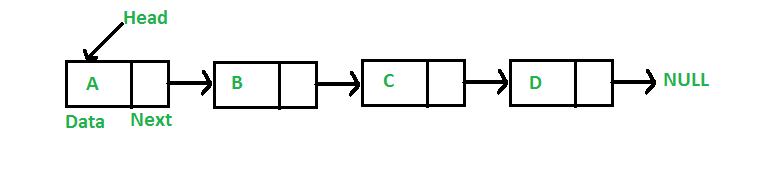
\includegraphics[scale=0.5]{linkedlist.png}
    \centering
\end{figure}
Nello \emph{stack} verrà mantenuto un puntatore che punta alla \textbf{testa} della \textbf{lista dinamica}.
Ogni nodo della lista avrà poi il puntatore all'elemento successivo.

~\newline
Esempio:
\begin{lstlisting}[language=C]
    #include <stdio.h>
    #include <stdlib.h>

    struct elem_{
        int num;
        struct elem_ *next;
    };
    typedef struct elem_ elem;  // rinomino il tipo

    elem * inserisciInCoda(elem *, int);
    void visualizza(elem *);

    int main(){

        return 0;
    }
\end{lstlisting}



\end{document}